\chapter{Laplace's method}
\label{ch:laplace}

In this chapter, we study an analytical tool to handle intractable Gibbs distributions: \emph{Laplace's method}. We use this method to analytically approximate the normalization constant of certain Gibbs distributions, which is often the main source of intractability. The essence of the method is to rewrite the normalization constant as an integral of the form
%
\begin{equation}
\int \exp\left(-\frac{1}{T}f(y)\right) dy,
\end{equation}
%
where $f$ is a convex function (or at least something similar to it). Afterwards, we exploit the fact that for sufficiently low $T$, this integral is approximated by $\exp(-\frac{1}{T}f(y_0))$, where $y_0$ is the minimum of $f$.

We illustrate this method in two scenarios. The first one is just a toy example. The second one shows how to cluster documents represented as vectors using the bag of words model. In this case, we wish then to cluster documents not by their Euclidean distance, but by how much the words occurring in the respective documents overlap. For two documents $x$ and $y$ represented as vectors, this overlap can be quantified by their \emph{cosine similarity}: $x^\top y / \left\|x\right\|\left\|y\right\|$.

\newpage
\section{Laplace's method}

\begin{theorem}
Let $f : \mathbb{R}^D \to \mathbb{R}$ be a twice continuously differentiable function. If $f$ has a unique minimum $y_0$ and $H := \frac{\partial^2 f}{\partial y^2} \bigr |_{y_0}$ (the Hessian of $f$ evaluated at $y_0$) is positive definite then
%
\begin{equation}
\lim_{M \to \infty} \frac{\displaystyle \int \exp\left(-M f(y)\right) dy}{\displaystyle \exp\left(-M f(y_0)\right)\left|\frac{MH}{2\pi}\right|^{-1/2}}=1.
\end{equation}
%
\label{thm:laplace}
\end{theorem}

Intuitively, Laplace's method suggests to approximate $\int \exp\left(-M f(y)\right) dy$ with $\exp\left(-M f(y_0)\right)$ if $M$ is sufficiently large.

Figure~\ref{fig:laplace} illustrates the behavior of $\exp\left(-M f(y)\right)$, with $f(y) = -1 + y^2 + \sin(5y)$. Observe that although $\int \exp\left(-M f(y)\right) dy$ is analytically intractable, as $M \to \infty$, the area under the curve is mostly around the minimum of $f$.

\begin{figure}[hbtp]
\centering
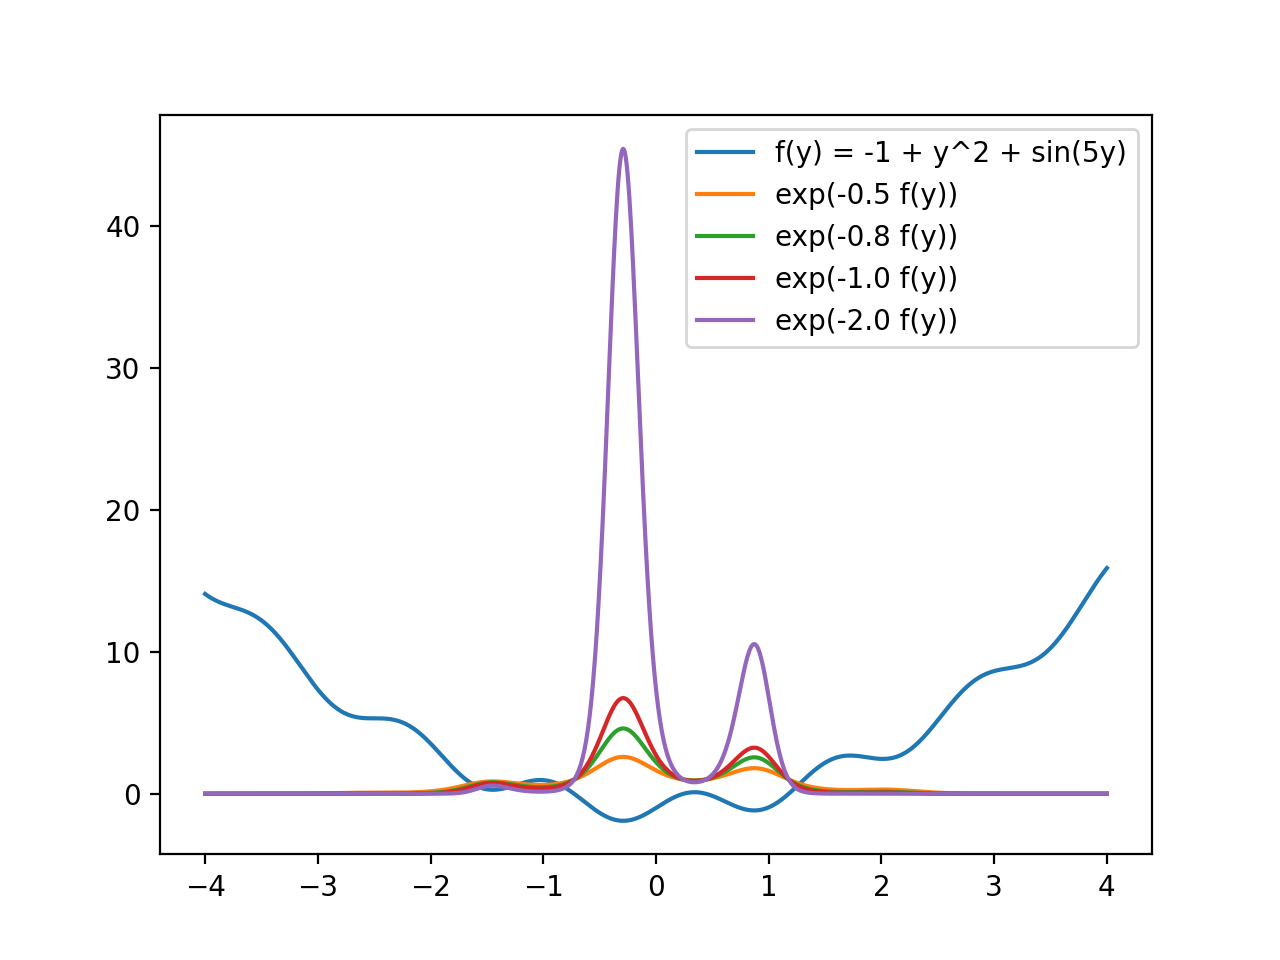
\includegraphics[width=\textwidth]{\dir/laplace.png}
\caption{}
\label{fig:laplace}
\end{figure}

The proof of Theorem~\ref{thm:laplace} relies on showing that
%
\begin{equation}
\lim_{M \to \infty} \frac{\displaystyle \int \exp\left(-M f(y)\right) dy}{\displaystyle \int \exp\left(-M T^2_f(y)\right) dy}=1,
\end{equation}
%
where $T^2_f(y)$ is the 2nd order Taylor approximation of $f$ at $y_0$ evaluated at $y$:
%
\begin{align}
T^2_f(y) &= f(y_0) + (y - y_0)^\top \frac{\partial f}{\partial y}\Bigr|_{y_0} + \frac{1}{2}(y - y_0)^\top H (y - y_0)\\
&= f(y_0) + \frac{1}{2}(y - y_0)^\top H (y - y_0).
\end{align}
%

\section{Illustrative example}

Let $\mathcal{C} = \{-1, +1\}^N$, for some $N \in \mathbb{N}$. We now illustrate how to exploit Laplace's method to approximate the intractable Gibbs distribution
%
\begin{equation}
p(c) := \frac{1}{Z}\exp\left(-\frac{1}{T}R(c)\right),
\end{equation}
%
where
%
\begin{equation}
Z := \sum_{c \in \mathcal{C}} \exp\left(-\frac{1}{T}R(c)\right) \qquad \text{and} \qquad R(c) := - \left(1 + \sum_{i \leq N}c_i\right)^2.
\end{equation}

The normalization constant is a sum over $2^N$ elements and becomes intractable for large $N$. The following exercises illustrate a recipe, formalized in Section~\ref{sec:laplace_recipe}, for approximating this constant using Laplace's method.

\begin{exercise}{[Square the cost]}
Show that
%
\begin{equation}
\exp\left(-\frac{1}{T}R(c)\right) = \exp\left(\frac{1}{T}\left(1 + \sum_{i \leq N}c_i\right)^2\right)
\end{equation}
%
\end{exercise}

\begin{exercise}{[Complete the square]}

Starting from here
%
\begin{equation}
\left(\pi T\right)^{1/2} = \int \exp\left(-\frac{1}{T}\left(y - \left(1 + \sum_{i \leq N}c_i\right)^2\right)\right)dy,
\end{equation}
%
show that
%
\begin{align*}
&\exp\left(\frac{1}{T}\left(1 + \sum_{i \leq N}c_i\right)^2\right)\\ 
&= \left(\pi T\right)^{-1/2}\int\exp\left(-\frac{1}{T}y^2 + \frac{2}{T}y\right) \prod_{i \leq N}\exp\left(\frac{2}{T}y c_i\right) dy.
\end{align*}
%
\end{exercise}

\begin{exercise}{[Rewrite normalization constant]}
Complete the following derivation
%
\begin{align}
Z &= \sum_{c} \exp\left(\frac{1}{T}\left(1 + \sum_{i \leq N}c_i\right)^2\right)\\ 
&= \left(\pi T\right)^{-1/2}\int\exp\left(-\frac{1}{T}y^2 + \frac{2}{T}y\right) \prod_{i \leq N}\exp\left(\frac{2}{T}y c_i\right) dy\\
&= \ldots \\
&= \left(\pi T\right)^{-1/2}\int \exp\left(-\frac{1}{T}f(y)\right) dy,\label{eq:norm_cost_ugly_integral}
\end{align}
%
where
%
\begin{equation}
f(y) = y^2 - 2 y - T N \log \left(2 \cosh\left(\frac{2}{T}y\right)\right).
\end{equation}
%
Hint: Apply Lemma~\ref{lem:sum_prod_exchange}. Recall also that
%
\begin{equation}
2 \cosh(x) = \exp(x) + \exp(-x).
\end{equation}
%
\end{exercise}

\begin{exercise}{[Apply Laplace's method]}
Show that $f$ has a unique global minimum at a point $y^*$ such that
%
\begin{equation}
y^* = 1 + N \tanh\left(\frac{2}{T}y^*\right).
\end{equation}
% 
Furthermore, show that $\frac{df}{dy}\bigr|_{y^*} > 0$ for sufficiently large $N$.
\end{exercise}

As a result, if we apply Laplace's method for sufficiently large $N$, the normalization constant can be approximated to $\exp\left(-\frac{1}{T}f(y^*)\right)$.
%
%\begin{equation}
%\left(\pi T\right)^{-3/2}\left(\frac{df}{dy}\bigr|_{y^*}\right)^{-1/2}\exp\left(-\frac{1}{T}f(y^*)\right).
%\end{equation}
%

\section{Using Laplace's method to approximate intractable normalization constants}
\label{sec:laplace_recipe}

The section before illustrates the following analytical strategy to estimate normalization constants:

\begin{enumerate}
\item \textbf{Square the cost} Rewrite your cost function as the squared norm of some vector, so that
%
\begin{equation}
\exp\left(-\frac{1}{T}R(c, X)\right) = \mathit{const}\exp\left(g(c)^\top g(c)\right).
\end{equation}
%
\item \textbf{Complete the square} Recall that
%
\begin{equation}
\pi^{d/2} = \int \exp\left(-\left\|y - g(c)\right\|^2\right) dy.
\end{equation}
%
Use this to derive that
%
\begin{equation}
\exp\left(g(c)^\top g(c)\right) = \pi^{-d/2}\int \exp\left(-y^\top y + 2y^\top g(c)\right)dy.
\end{equation}
%
\item \textbf{Rewrite the normalization constant} Show that the normalization constant can be expressed as follows
%
\begin{align}
Z &= \sum_{c} \exp\left(-\frac{1}{T}R(c, X)\right)\\ 
&= \ldots\\
&= \mathit{const} \int \exp\left(-M f(y)\right)dy.
\end{align}
%

\item \textbf{Apply Laplace's method} Verify that the conditions for Laplace's method hold and apply it to estimate $Z$ with $\mathit{const}\exp\left(-M f(y_0)\right)$, where $y_0$ is the minimum of $f$.
\end{enumerate}

\section{Least-angle clustering}

We now apply Laplace's method for a more interesting problem.
Assume given a set $X = \{x_1, x_2, \ldots, x_N\} \subseteq \mathbb{R}^d$ of unit vectors. We wish to cluster them in $K$ clusters so that any pair of vectors are assigned to the same cluster if they point in similar directions.

We model a cluster assignment as a matrix $M \in \{0, 1\}^{N \times K}$, where
%
\begin{equation}
M_{ik} \begin{cases}
1 & \text{if $x_i$ is assigned to cluster $k$}\\
0 & \text{otherwise}.
\end{cases}
\end{equation}
%
Therefore, it is required that $\sum_{k \leq K} M_{ik} = 1$, for any $i \leq N$. Observe that for $i, j \leq N$ and $k \leq K$, $M_{ik}M_{jk} = 1$ iff $x_i$ and $x_j$ are assigned to the same cluster.\looseness=-1

Our goal is to use maximum entropy to train a cluster assignment, using the following cost function
%
\begin{equation}
R(M, X) = -\frac{1}{N}\sum_{i < j \leq N} \sum_{k \leq K} M_{ik}M_{jk}x_i^\top x_j.
\end{equation}
%

Observe that the normalization constant of the Gibbs distribution induced by this cost function is a sum over $K^N$ elements, making it intractable. The next four sections illustrate how to manipulate the normalization constant so we can apply Laplace's method.

%\section{Outline}
%
%We first rewrite the cost function into a sum, where each term in the sum is a quadratic form. Afterwards, we introduce dummy variables and use the technique of completing the square to 

\section{Square the cost}
\label{sec:cost_function_la}

\begin{exercise}
Show that
%
\begin{equation}
R(M, X) = -\frac{1}{2N}\sum_{k \leq K}\left\|\sum_{i \leq N} M_{ik}x_i\right\|^2 + \frac{1}{2}.
\end{equation}
\label{ex:cost_fun_quad}
\end{exercise}

\begin{proof}
%
Observe that, $M^2_{ik} = M_{ik}$, since $M_{ik} \in \{0, 1\}$. Furthermore, $x_i^\top x_i = 1$, as $x_i$ is a unit vector, for $i \leq N$. We now prove this auxiliary result.
%
\begin{align}
\sum_{k \leq K} \sum_{i \leq N} M_{ik}^2x_i^\top x_i
= \sum_{k \leq K} \sum_{i \leq N} M_{ik}^2
&= \sum_{k \leq K} \sum_{i \leq N} M_{ik}\\ 
&= \sum_{i \leq N}\sum_{k \leq K}M_{ik}\\\
&= \sum_{i \leq N} 1\\
&= N.
\end{align}

We now prove the claim.
%
\begin{align}
&- \frac{1}{2N}\sum_{k \leq K}\left\|\sum_{i \leq N} M_{ik}x_i\right\|^2 + \frac{1}{2}\\
&= -\frac{1}{2N}\sum_{k \leq K}\left(2\sum_{i < j \leq N}M_{ik}M_{jk}x_i^\top x_j^\top + \sum_{i \leq N} M_{ik}^2 x_i^\top x_i\right) + \frac{1}{2}\\
&= -\frac{1}{N}\sum_{k \leq K}\sum_{i < j \leq N}M_{ik}M_{jk}x_i^\top x_j^\top -\frac{1}{2N}\sum_{k \leq K} \sum_{i \leq N} M_{ik}^2 x_i^\top x_i + \frac{1}{2}\\
&= -\frac{1}{N}\sum_{k \leq K}\sum_{i < j \leq N}M_{ik}M_{jk}x_i^\top x_j^\top -\frac{1}{2} + \frac{1}{2} = R(M, X)
\end{align}
%%
%\begin{align}
%R(M, X) &= -2\left(\frac{1}{2N}\sum_{i < j \leq N} \sum_{k \leq K} M_{ik}M_{jk}x_i^\top x_j\right)\\
%&= -\frac{1}{2N}\sum_{i < j \leq N} \sum_{k \leq K} M_{ik}M_{jk}x_i^\top x_j -\frac{1}{2N}\sum_{i < j \leq N} \sum_{k \leq K} M_{ik}M_{jk}x_i^\top x_j\\
%&= -\frac{1}{2N}\sum_{i < j \leq N} \sum_{k \leq K} M_{ik}M_{jk}x_i^\top x_j -\frac{1}{2N}\sum_{j < i \leq N} \sum_{k \leq K} M_{ik}M_{jk}x_i^\top x_j\\
%&= -\frac{1}{2N}\sum_{i < j \leq N} \sum_{k \leq K} M_{ik}M_{jk}x_i^\top x_j-\frac{1}{2N}\sum_{j < i \leq N} \sum_{k \leq K} M_{ik}M_{jk}x_i^\top x_j+\\
%& -\frac{1}{2N}\sum_{i} \sum_{k \leq K} M_{ik}M_{ik}x_i^\top x_i+\frac{1}{2N}\sum_{i} \sum_{k \leq K} M_{ik}M_{ik}x_i^\top x_i\\
%&= -\frac{1}{2N}\sum_{k \leq K}\sum_{i, j \leq N}  M_{ik}M_{jk}x_i^\top x_j + \frac{1}{2N}\sum_{i} \sum_{k \leq K} M_{ik}M_{ik}x_i^\top x_i\\
%&= - \frac{1}{2N}\sum_{k \leq K}\sum_{i, j \leq N} M_{ik}M_{jk} x_i^\top x_j + \frac{1}{2N}N.\\
%&= - \frac{1}{2N}\sum_{k \leq K}\sum_{i, j \leq N} M_{ik}M_{jk} x_i^\top x_j + \frac{1}{2}.\\
%&= - \frac{1}{2N}\sum_{k \leq K}\left\|\sum_{i \leq N} M_{ik}x_i\right\|^2 + \frac{1}{2}.
%\end{align}
%
\end{proof}

This result only implies that
%
\begin{equation}
\exp\left(-\frac{1}{T}R(M, X)\right) = e^{-\frac{1}{2T}}\prod_{k \leq K}\exp\left(-\frac{1}{2N}\left\|\sum_{i \leq N}M_{ik}x_i\right\|^2\right).
\end{equation}
%
This is not an expression of the form $\textit{const} \exp\left(g(c)^\top g(c)\right)$, as recommended in Section~\ref{sec:laplace_recipe}. However, we show next how to adapt the cost function so that we can still follow all the other steps from Section~\ref{sec:laplace_recipe}.

\section{Complete the square}

Recall the Gibbs distribution
%
$$p(c \mid X) = \frac{1}{Z_X}\exp\left(-\frac{1}{T}R(M, X)\right),$$
%
where $Z_X$ is the partition function. 

\begin{exercise}
Prove that
%
\begin{equation}
Z_X = \sum_{M \in \{0, 1\}^{N \times K}}e^{-\frac{1}{2T}}\prod_{k \leq K} \exp\left(\frac{1}{2NT}\left\|\sum_{i \leq N} M_{ik}x_i\right\|^2\right).
\label{eq:partition_function}
\end{equation}
%
\end{exercise}

\begin{proof}
\begin{align*}
Z_X &= \sum_{M} \exp\left(-\frac{1}{T}R(M, X)\right)\\
&= \sum_{M} \exp\left(\frac{1}{2NT}\sum_{k \leq K}\left\|\sum_{i \leq N} M_{ik}x_i\right\|^2 - \frac{1}{2T}\right)\\
&= e^{-\frac{1}{2T}}\sum_{M} \prod_{k \leq K}\exp\left(\frac{1}{2NT}\left\|\sum_{i \leq N} M_{ik}x_i\right\|^2\right).\\
\end{align*}
\end{proof}

Observe that the partition function requires to compute a sum over $2^{N \times K}$ elements and it is not clear how to do that sum analytically or in a computationally efficient way. Hence, computing the Gibbs distribution takes exponential time. This makes ME + PA very inefficient as these methods rely on computing the Gibbs distribution.

We now use the technique of completing the square.

\begin{exercise}
For $k \leq K$, define a dummy variable $y_k$. Show that
%
\begin{align}
&exp\left(\frac{1}{2NT}\left\|\sum_{i \leq N} M_{ik}x_i\right\|^2\right)\\
&\qquad = \left(\frac{2\pi T}{N}\right)^{-\frac{D}{2}} \int \exp\left(- \frac{N}{2T}\left\|y_k\right\|^2 + \frac{1}{T}\sum_{i \leq N}M_{ik}x_i^\top y_k\right)dy_k
\label{eq:partition_trick}
\end{align}
%
\textit{Hint: Start from here
%
$$\int \exp\left(-\frac{N}{2T} \left\|y_k - \frac{1}{N}\sum_{i \leq N}M_{ik}x_i\right\|^2\right)dy_k.$$
%
Observe that this is the normalization constant for a multivariate Gaussian distribution.}
\end{exercise}

\begin{proof}
Using the fact that this is the normalization constant of a Gaussian, we have that
%
\begin{align}
&\left(\frac{2\pi T}{N}\right)^{\frac{D}{2}}\\
 &= \int \exp\left(-\frac{N}{2T} \left\|y_k - \frac{1}{N}\sum_{i \leq N}M_{ik}x_i\right\|^2\right)dy_k\\
&= \int \exp\left(-\frac{N}{2T}\left[ \left\|y_k\right\|^2 - \frac{2}{N}y_k^\top\sum_{i \leq N}M_{ik}x_i + \frac{1}{N^2}\left\|\sum_{i \leq N}M_{ik}x_i\right\|^2\right]\right)dy_k\\
&= \exp\left(-\frac{N}{2T}\frac{1}{N^2}\left\|\sum_{i \leq N}M_{ik}x_i\right\|^2\right)\int \exp\left(-\frac{N}{2T}\left[ \left\|y_k\right\|^2 - \frac{2}{N}y_k^\top\sum_{i \leq N}M_{ik}x_i\right]\right)dy_k\\
&= \exp\left(-\frac{1}{2NT}\left\|\sum_{i \leq N}M_{ik}x_i\right\|^2\right)\int \exp\left(-\frac{N}{2T}\left\|y_k\right\|^2 +\frac{1}{T}y_k^\top\sum_{i \leq N}M_{ik}x_i\right)dy_k.
\end{align}
%
We can rearrange the resulting equation to obtain Equation~\ref{eq:partition_trick}.
\end{proof}

\section{Rewrite the normalization constant}
\label{sec:swap_sum_prod}

\begin{exercise}
Using Equations~\ref{eq:partition_function} and~\ref{eq:partition_trick}, show that
%
\begin{equation}
Z_X = \alpha \int\exp\left(-\frac{N}{2T}\sum_{k \leq K} \left\|y_k\right\|^2 + \sum_{i \leq N} \log \sum_{k \leq K} \exp\left(\frac{1}{T}x_i^\top y_k\right)\right)d\mathbf{y},
\end{equation}
%
where
%
\begin{align}
\alpha &:= e^{-\frac{1}{2T}}\left(\frac{2\pi T}{N}\right)^{-\frac{KD}{2}}, \text{ and}\\
\int g(y_1, \ldots, y_K)d\mathbf{y} &:= \int \int \ldots \int g(y_1, \ldots, y_K) dy_1 dy_2\ldots dy_K.
\end{align}

\textit{Hint: Prove and use the following auxiliary results.}

$$\prod_{k \leq K} \int f_k(y_k) dy_k = \int \prod f_k(y_k) d\mathbf{y}.$$

$$\sum_{M \in \{0, 1\}^{N \times K}}\prod_{i \leq N}\exp\left(\frac{1}{T}\sum_{k \leq K}M_{ik}x_i^\top y_k\right) = \prod_{i \leq N}\sum_{k \leq K}\exp\left(\frac{1}{T}x_i^\top y_k\right).$$
\end{exercise}

\begin{proof}
Using Equation~\ref{eq:partition_trick}, Equation~\ref{eq:partition_function} becomes
%
\begin{align}
Z_X &= e^{-\frac{1}{2T}}\sum_{M \in \{0, 1\}^{N \times K}}\prod_{k \leq K} \exp\left(\frac{1}{2NT}\left\|\sum_{i \leq N} M_{ik}x_i\right\|^2\right)\\
&= e^{-\frac{1}{2T}}\sum_{M \in \{0, 1\}^{N \times K}}\prod_{k \leq K} \left(\frac{2\pi T}{N}\right)^{\frac{D}{2}} \int \exp\left(- \frac{N}{2T}\left\|y_k\right\|^2 + \frac{1}{T}\sum_{i \leq N}M_{ik}x_i^\top y_k\right)dy_k\\
&= e^{-\frac{1}{2T}}\left(\frac{2\pi T}{N}\right)^{\frac{KD}{2}}\sum_{M \in \{0, 1\}^{N \times K}}\prod_{k \leq K}  \int \exp\left(- \frac{N}{2T}\left\|y_k\right\|^2 + \frac{1}{T}\sum_{i \leq N}M_{ik}x_i^\top y_k\right)dy_k.
\end{align}

Observe now the following property.
%
\begin{align*}
\prod_{k \leq K} \int f_k(y_k) dy_k &= \left(\int f_1(y_1) dy_1\right)\left(\int f_2(y_2) dy_2\right)\ldots \left(\int f_K(y_K) dy_K\right)\\
&= \int f_1(y_1) f_2(y_2) \ldots f_K(y_K) d\mathbf{y}\\
&= \int \prod f_k(y_k) d\mathbf{y}.
\end{align*}

Applying this property above gives us the following.

\begin{align}
&Z_X\\
&= \alpha\sum_M\int \prod_{k \leq K} \exp\left(- \frac{N}{2T}\left\|y_k\right\|^2 + \frac{1}{T}\sum_{i \leq N}M_{ik}x_i^\top y_k\right)d\mathbf{y}\\
&= \alpha\sum_M\int \exp\left(- \frac{N}{2T}\sum_{k \leq K}\left\|y_k\right\|^2 + \frac{1}{T}\sum_{k \leq K}\sum_{i \leq N}M_{ik}x_i^\top y_k\right)d\mathbf{y}\\
&= \alpha\sum_M\int \exp\left(- \frac{N}{2T}\sum_{k \leq K}\left\|y_k\right\|^2\right)\exp\left(\frac{1}{T}\sum_{i \leq N}\sum_{k \leq K}M_{ik}x_i^\top y_k\right)d\mathbf{y}\\
&= \alpha\sum_M\int \exp\left(- \frac{N}{2T}\sum_{k \leq K}\left\|y_k\right\|^2\right)\prod_{i \leq N}\exp\left(\frac{1}{T}\sum_{k \leq K}M_{ik}x_i^\top y_k\right)d\mathbf{y}\\
&= \alpha\int \sum_{M}\left[\exp\left(- \frac{N}{2T}\sum_{k \leq K}\left\|y_k\right\|^2\right)\prod_{i \leq N}\exp\left(\frac{1}{T}\sum_{k \leq K}M_{ik}x_i^\top y_k\right)\right]d\mathbf{y}\\
&= \alpha\int \exp\left(- \frac{N}{2T}\sum_{k \leq K}\left\|y_k\right\|^2\right)\sum_{M}\prod_{i \leq N}\exp\left(\frac{1}{T}\sum_{k \leq K}M_{ik}x_i^\top y_k\right)d\mathbf{y}.
\end{align}

We now apply Lemma~\ref{lem:sum_prod_exchange}. To do this, given $M \in \{0, 1\}^{N \times K}$, we define an auxiliary function $c_M : \{1, \ldots, N\} \to \{1, \ldots, K\}$. For $i \leq N$, $c_M(i) = k$ iff $M_{ik} = 1$. Observe that $c_M$ is well defined as $M \in \{0, 1\}^{N \times K}$ and $\sum_k M_{ik} = 1$. As a result, $\sum_k {M_{ik}}x_i^\top y_k = x_i^\top y_{c(i)}$. Observe then the following:
%
\begin{align}
&\sum_{M \in \{0, 1\}^{N \times K}}\prod_{i \leq N}\exp\left(\frac{1}{T}\sum_{k \leq K}M_{ik}x_i^\top y_k\right) \\
&= \sum_{c : \{1, \ldots, N\} \to \{1, \ldots, K\}}\prod_{i \leq N}\exp\left(\frac{1}{T}x_i^\top y_{c(i)}\right)\\
&= \prod_{i \leq N}\sum_{k \leq K}\exp\left(\frac{1}{T}x_i^\top y_k\right).
\end{align}
% 

If we apply this to the equation above, we get

\begin{align}
&Z_X\\
 &= \alpha\int \exp\left(- \frac{N}{2T}\sum_{k \leq K}\left\|y_k\right\|^2\right)\prod_{i \leq N}\sum_{k \leq K}\exp\left(\frac{1}{T}x_i^\top y_k\right)d\mathbf{y}\\
&= \alpha\int \exp\left(- \frac{N}{2T}\sum_{k \leq K}\left\|y_k\right\|^2\right)\exp\left(\log\left(\prod_{i \leq N}\sum_{k \leq K}\exp\left(\frac{1}{T}x_i^\top y_k\right)\right)\right)d\mathbf{y}\\
&= \alpha\int \exp\left(- \frac{N}{2T}\sum_{k \leq K}\left\|y_k\right\|^2 + \sum_{i \leq N}\log\sum_{k \leq K}\exp\left(\frac{1}{T}x_i^\top y_k\right)\right)d\mathbf{y}\label{eq:monster_integral}
\end{align}
\end{proof}

\section{Apply Laplace's method}

%The integral in Equation~\ref{eq:monster_integral} is analytically intractable. However, it can be expressed in the form $\exp\left(-\frac{N}{T}f_X(y_1, \ldots, y_K)\right)$, where $f_X$ has a unique minimum at 0. This allows us to use what is called \emph{the Laplace method}, a method to approximate the integral with arbitrary precision as $\frac{N}{T} \to \infty$.

Let $\mathbf{y}$ be the vector of real variables resulting from the concatenation of $y_1, y_2, \ldots, y_k$. Equation~\ref{eq:monster_integral} can then be rewritten as
%
\begin{equation}
Z_X = e^{-\frac{1}{2T}}\left(\frac{2\pi T}{N}\right)^{-\frac{KD}{2}}\int \exp\left( - \frac{N}{T}f_X(\mathbf{y}) \right)d\mathbf{y},
\end{equation}
%
where
%
\begin{equation}
f_X(\mathbf{y}) = \frac{1}{2}\sum_{k \leq K}\left\|y_k\right\|^2 - \frac{T}{N}\sum_{i \leq N}\log\sum_{k \leq K}\exp\left(\frac{1}{T}x_i^\top y_k\right).
\end{equation}

The exercises below show that when $T > 1$, the Hessian of $f_X$ evaluated at any point is positive definite. Therefore, $f_X$ has a unique global minimum and $H$, the Hessian evaluated at that minimum, is positive definite. We can then estimate $Z_X$ with
%
\begin{equation}
Z_X \approx e^{-\frac{1}{2T}}\left(\frac{2\pi T}{N}\right)^{-\frac{KD}{2}}\left|\frac{NH}{2\pi T}\right|^{-\frac{1}{2}}.
\end{equation}
%

%
%Recall now that $f_X(\mathbf{y})$'s second-order Taylor expansion at $\mathbf{y}^* \in \mathbb{R}^{KD}$ is given by
%%
%$$f_X(\mathbf{y}) \approx f_X(\mathbf{y}^*) + (\mathbf{y} - \mathbf{y}*)^\top \left.\frac{\partial f_X}{\partial \mathbf{y}}\right|_{\mathbf{y}^*} + (\mathbf{y} - \mathbf{y}^*)^\top \left.\frac{\partial^2 f_X}{\partial \mathbf{y}^2}\right|_{\mathbf{y}^*}(\mathbf{y} - \mathbf{y}^*),$$
%%
%where $\left.\frac{\partial f_X}{\partial \mathbf{y}}\right|_{\mathbf{y}^*}$ is $f_X$'s gradient evaluated at $\mathbf{y}^*$ and $\left.\frac{\partial^2 f_X}{\partial \mathbf{y}^2}\right|_{\mathbf{y}^*}$ is $f_X$'s Hessian evaluated at $\mathbf{y}^*$.
%
%If we choose $\mathbf{y}^*$ to be $f_X's$' minimum, then this reduces to
%%
%$$f_X(\mathbf{y}) \approx f_X(\mathbf{y}^*) + (\mathbf{y} - \mathbf{y}^*)^\top \left.\frac{\partial^2 f_X}{\partial \mathbf{y}^2}\right|_{\mathbf{y}^*}(\mathbf{y} - \mathbf{y}^*).$$
%%
%
%\begin{exercise}
%Using this approximation, and assuming that $\mathbf{y}^*$ and that $\left.\frac{\partial^2 f_X}{\partial \mathbf{y}^2}\right|_{\mathbf{y}^*}$ are given, show that
%%
%$$Z_X \approx \left(\frac{2\pi T}{N}\right)^{\frac{KD}{2}} \left(2\pi\right)^{D/2}\left|\left.\frac{\partial^2 f_X}{\partial \mathbf{y}^2}\right|_{\mathbf{y}^*}\right|^{-\frac{1}{2}}\exp\left(-\frac{1}{2T}-\frac{N}{T}f_X(\mathbf{y}^*)\right).$$
%%
%\end{exercise}
%
%\begin{proof}
%\begin{align*}
%Z_X &= e^{-\frac{1}{2T}}\left(\frac{2\pi T}{N}\right)^{\frac{KD}{2}}\int \exp\left( - \frac{N}{T}f_X(\mathbf{y}) \right)d\mathbf{y}\\
%&\approx e^{-\frac{1}{2T}}\left(\frac{2\pi T}{N}\right)^{\frac{KD}{2}}\int \exp\left( - \frac{N}{T}\left(f_X(\mathbf{y}^*) + (\mathbf{y} - \mathbf{y}^*)^\top \left.\frac{\partial^2 f_X}{\partial \mathbf{y}^2}\right|_{\mathbf{y}^*}(\mathbf{y} - \mathbf{y}^*)\right) \right)d\mathbf{y}\\
%&= e^{-\frac{1}{2T}}\left(\frac{2\pi T}{N}\right)^{\frac{KD}{2}}\exp\left( - \frac{N}{T}f_X(\mathbf{y}^*)\right)\int \exp\left((\mathbf{y} - \mathbf{y}^*)^\top \left.\frac{\partial^2 f_X}{\partial \mathbf{y}^2}\right|_{\mathbf{y}^*}(\mathbf{y} - \mathbf{y}^*)\right) d\mathbf{y}\\
%&= e^{-\frac{1}{2T}}\left(\frac{2\pi T}{N}\right)^{\frac{KD}{2}}\exp\left( - \frac{N}{T}f_X(\mathbf{y}^*)\right)\int \exp\left(-\frac{1}{2}(\mathbf{y} - \mathbf{y}^*)^\top \left(-2\left.\frac{\partial^2 f_X}{\partial \mathbf{y}^2}\right|_{\mathbf{y}^*}\right)(\mathbf{y} - \mathbf{y}^*)\right) d\mathbf{y}\\
%&= e^{-\frac{1}{2T}}\left(\frac{2\pi T}{N}\right)^{\frac{KD}{2}}\exp\left( - \frac{N}{T}f_X(\mathbf{y}^*)\right)\left|2\pi\left.\frac{\partial^2 f_X}{\partial \mathbf{y}^2}\right|_{\mathbf{y}^*}^{-1}\right|^{\frac{1}{2}}\\
%&= e^{-\frac{1}{2T}}\left(\frac{2\pi T}{N}\right)^{\frac{KD}{2}}\exp\left( - \frac{N}{T}f_X(\mathbf{y}^*)\right)\left|2\pi\left.\frac{\partial^2 f_X}{\partial \mathbf{y}^2}\right|_{\mathbf{y}^*}^{-1}\right|^{\frac{1}{2}}\\
%&= \left(\frac{2\pi T}{N}\right)^{\frac{KD}{2}} \left(2\pi\right)^{D/2}\left|\left.\frac{\partial^2 f_X}{\partial \mathbf{y}^2}\right|_{\mathbf{y}^*}\right|^{-\frac{1}{2}}\exp\left(-\frac{1}{2T}-\frac{N}{T}f_X(\mathbf{y}^*)\right).
%\end{align*}
%\end{proof}

The conditions for Laplace's method still hold for $T \leq 1$, but the proof is more involved and is left for a future version of the script.

\begin{exercise}
Show how to estimate $\mathbf{y}^*$, the minimum of $f_X$.
\end{exercise}

\begin{proof}
We obtain $\mathbf{y}^*$ by solving
%
\begin{equation}
\frac{\partial f_X}{\partial \mathbf{y}}= 0 \qquad \Leftrightarrow \qquad \frac{\partial f_X}{\partial y_k} = 0\text{, for all $k \leq K$}.
\end{equation}
%

\begin{align*}
\frac{\partial f_X}{\partial y_k} &= \frac{1}{2}\frac{\partial f_X}{\partial y_k}\sum_{k \leq K}\left\|y_k\right\|^2 - \frac{T}{N}\sum_{i \leq N}\frac{\partial f_X}{\partial y_k}\log\sum_{k \leq K}\exp\left(\frac{1}{T}x_i^\top y_k\right)\\
&= y_k - \frac{T}{N}\sum_{i \leq N}\frac{\frac{1}{T}x_i\exp\left(\frac{1}{T}x_i^\top y_k\right)}{\sum_{k' \leq K}\exp\left(\frac{1}{T}x_i^\top y_{k'}\right)}\\
\end{align*}
%
Hence, for $k \leq K$, $\frac{\partial f_X}{\partial y_k}= 0$ implies that 
%
$$y_k = \sum_{i \leq N}\frac{x_i\exp\left(\frac{1}{T}x_i^\top y_k\right)}{N\sum_{k' \leq K}\exp\left(\frac{1}{T}x_i^\top y_{k'}\right)}.$$
%
A solution for this transcendental equation can be approximated iteratively, using an EM-like procedure.
\end{proof}

\begin{exercise}
Show how to compute the Hessian matrix $\frac{\partial^2 f_X}{\partial \mathbf{y}^2}$.
\end{exercise}

\begin{proof}
Recall that for a function $g : \mathbb{R}^d \to \mathbb{R}$, the Hessian is defined as a matrix whose $(i,j)$ entry is $\frac{\partial^2 g}{\partial y_i \partial y_j}$. Hence, $\frac{\partial^2 f_X}{\partial \mathbf{y}^2}$ is the following block matrix:
%
$$\frac{\partial^2 f_X}{\partial \mathbf{y}^2} = 
\left(
\begin{array}{ccccc}
\frac{\partial^2 f_X}{\partial y_1 \partial y_1} && \ldots && \frac{\partial^2 f_X}{\partial y_1 \partial y_K}\\
& \ddots & & \reflectbox{$\ddots$} & \\
\vdots && \frac{\partial^2 f_X}{\partial y_k \partial y_\ell} && \vdots \\
& \reflectbox{$\ddots$} & & \ddots & \\
\frac{\partial^2 f_X}{\partial y_K \partial y_1} && \ldots && \frac{\partial^2 f_X}{\partial y_K \partial y_K}\\
\end{array}
\right).$$
%
Please be careful to observe that $\frac{\partial^2 f_X}{\partial y_k \partial y_\ell}$ is a \emph{matrix}! In particular, if $k = \ell$, then one can show that
%
\begin{equation}
\frac{\partial^2 f_X}{\partial y_k^2} = I - \frac{1}{TN}\sum_{i \leq N} x_i x_i^\top P_{ik} + \frac{1}{TN}\sum_{i \leq N} x_i x_i^\top P^2_{ik},
\end{equation}
%
where 
%
\begin{equation}
P_{ik} = \frac{\exp\left(\frac{1}{T}x_i^\top y_k\right)}{\sum_k \exp\left(\frac{1}{T}x_i^\top y_k\right)}.
\end{equation}
%
When $k \neq \ell$, one can show that
%
\begin{equation}
\frac{\partial^2 f_X}{\partial y_k \partial y_\ell} = \frac{1}{TN}\sum_{i \leq N} x_i x_i^\top P_{ik}P_{i\ell}.
\end{equation}
%
\end{proof}

\begin{exercise}
Show that if $T > 1$, then the Hessian is positive definite at any point.
\end{exercise}

\begin{proof}
Let $z = \left(z_1, \ldots, z_K\right)$. Observe that
%
\begin{align}
z^\top \frac{\partial^2 f_X}{\partial \mathbf{y}^2} z &= \sum_{k \leq K} \left(z_k^\top z_k - \frac{1}{TN}\sum_{i \leq N}z_k^\top x_i x_i^\top z_k P_{ik}\right) +\\
& \sum_{k, \ell \leq K} z_k^\top\left(\frac{1}{TN}\sum_{i \leq N}x_ix_i^\top P_{ik}P_{i\ell}\right)z_\ell\\
&= \sum_{k \leq K} \left(z_k^\top z_k - \frac{1}{TN}\sum_{i \leq N}z_k^\top x_i x_i^\top z_k P_{ik}\right) +\\
& \frac{1}{TN}\sum_i\left(\sum_{k} z_kP_{ik}\right)^\top x_ix_i^\top \left(\sum_{k} z_kP_{ik}\right)\\
&\geq \sum_{k \leq K} \left(z_k^\top z_k - \frac{1}{TN}\sum_{i \leq N}z_k^\top x_i x_i^\top z_k P_{ik}\right)\\
&= \sum_{k \leq K} z_k^\top z_k - \frac{1}{TN}\sum_{i \leq N}\sum_{k}P_{ik}z_k^\top x_i x_i^\top z_k\\
&\geq \sum_{k \leq K} z_k^\top z_k - \frac{1}{TN}\sum_{i \leq N}\sum_{k}z_k^\top z_k.
\end{align}

The last inequality follows from the fact that $P_{ik} \leq 1$ and that any entry of $x_ix_i^\top$ is at most 1 as $x_i$ is a unit vector, for $i \leq N$. Observe that if $T > 1$, then the right hand side is positive. This implies that the Hessian is positive definite at any point, when $T > 1$.
%
\end{proof}

%It can be shown that $\left.\frac{\partial^2 f_X}{\partial \mathbf{y}^2}\right|_{\mathbf{y}^*}$ is positive definite, when $T > 1$. One can then apply Laplace's method to do the following approximation:
%%
%\begin{equation}
%Z_X = e^{-\frac{1}{2T}}\left(\frac{2\pi T}{N}\right)^{\frac{KD}{2}}\exp\left( - \frac{N}{T}f_X(\mathbf{y^*}) \right).
%\end{equation}

%\section{Conclusion}
%
%In this section, we studied an analytical technique for approximating certain normalization constants. The technique works in four steps:
%
%\begin{enumerate}
%\item Write the cost $R(c, X)$ as the squared norm $g(c)^\top g(c)$ of some function $g$.
%\item Use the normalization constant of a Gaussian to rewrite the term $\exp\left(-\frac{1}{T}R(c, X)\right)$
%\end{enumerate}